\documentclass{article}
\usepackage{graphicx}
\begin{document}
\title{Specialized Cost Function for Maximizing Body Area Networks Lifetime Using Global Routing Algorithms}
\author{Alvaro Prieto}
\maketitle

\begin{abstract}
$\ll$ at the end $\gg$
\end{abstract}

\section{Introduction}
Wireless Body Area Networks (WBANs) consist of several wireless sensors located around a human body. These sensors may measure several biological signals, movement, and temperature. Due to major improvements in power consumption and constantly shrinking devices, WBANs are becoming ubiquitous. Due to the small form factor of these devices, the battery size is limited. While the sensors themselves may be extremely power efficient, all of the measured data must be transmitted over a much less efficient wireless link. One benefit of WBANs is that they rarely include more than a dozen wireless devices over a small area. This constraint allows for the use of routing techniques not suitable for larger wireless sensor networks.

There are several routing protocols designed specifically for WBANs. Braem et al. developed the CICADA protocol, which consists of a spanning tree architecture with a time-division scheme for transmission scheduling~\cite{protocol:CICADA}. The primary downside to this method is that nodes closer to the root will deplete their energy source faster due to the need to relay messages from children nodes. Other protocols focus on the reliability of the network~\cite{routing:storeandforward}. Dynamic networks are a problem with WBANs. If sensors are placed in the extremities, the network will change as the body changes positions. Quwaider et al. developed a protocol tolerant to network changes~\cite{routing:storeandforward}. They propose a store-and-forward method that maximizes the likelihood of a packet reaching its destination. Each packet is stored by multiple devices and retransmitted, which consumes more power. One solution for this problem was proposed by Ehyaie et al.~\cite{relay:networklife}, it consists of using dedicated, non-sensing, relay nodes with larger power sources. While this method increases the network lifetime$\ll$define term$\gg$, it requires more hardware. Finally, Nabi et al. propose a similar store-and-forward method, but integrates Transmit Power Adaptation (TPA)~\cite{relay:transmitpoweradaptation}. Nodes keep track of neighbors and use power control to use the smallest transmit power while maintaining a specific link quality.

In this contribution we propose a novel routing algorithm that focuses not on single devices, but the overall network. Current methods focus on maximizing device lifetime. This is generally a good goal, but certain systems require all devices working to function properly. Keeping that in mind, the proposed system maximizes the network lifetime by normalizing power use across the network.
$\ll$”In this contribution we …. (elaborate on title), describe the algorithm (“in contradistinction to previous routing approached, we define a cost function based on the deviation of the accumulated energy of a single node from the overall average power…”), summary of work (real RSSI data + simulation and hardware implementation using TI 2.4, comparison approach, network lifetime and energy per bit…), summary of results.”$\gg$ 

\begin{figure}[htb]
\begin{center}
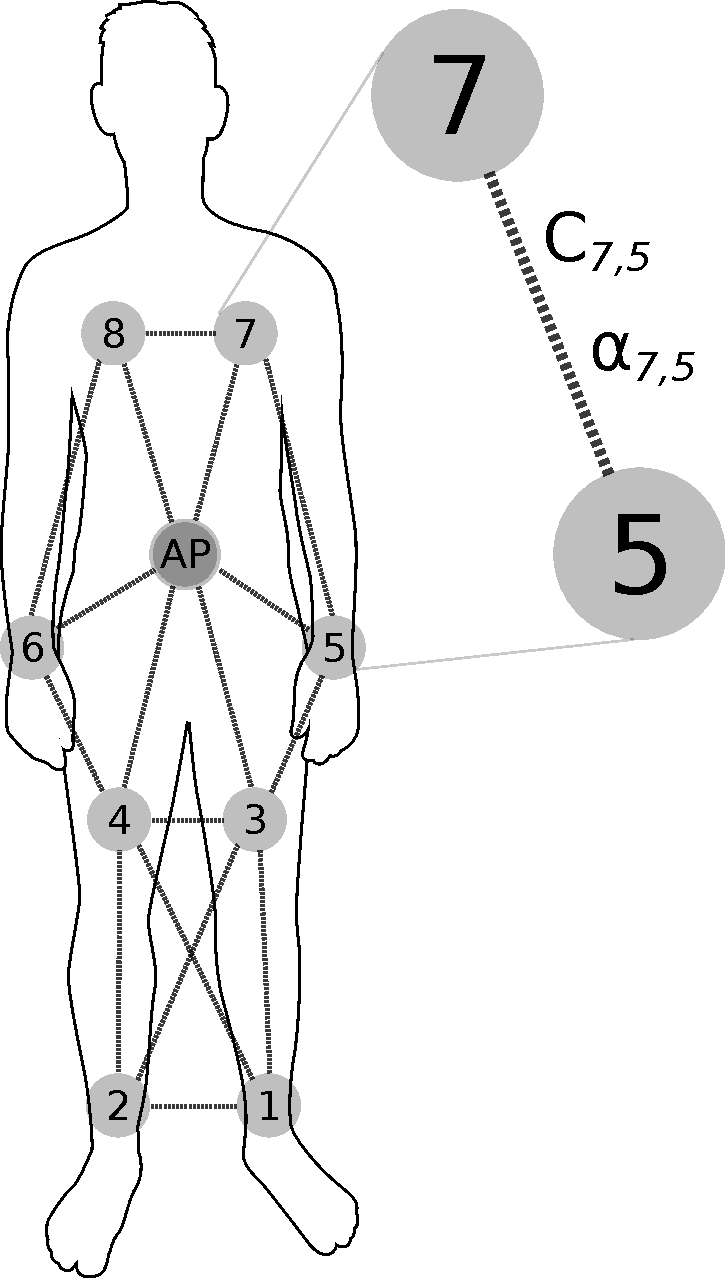
\includegraphics[width=0.5\textwidth]{figures/body.pdf}
\end{center}
\caption{Experimental Setup}
\label{fig:body}
\end{figure}

\section{Proposed Cost Function}
In the proposed system, we define a new link cost function that is then used in the routing algorithm. Traditionally, the power required to make a link possible is used as the link cost. In this case, the total energy used by a device is factored into the equation. If a device has used more energy than the others, its use as a relay will be discouraged.

Each device's energy use is accumulated as shown in Equation~\ref{eqn:accumulated_energy}, where $j$ denotes the device ID, $i$ is the current polling round, $\alpha$ is the channel attenuation, and $RSSI^T$ is the target RSSI. The current energy used is incremented by the energy used to transmit a single packet while maintaining $RSSI^T$. The channel attenuation for the selected link,$\alpha$, can be seen in Equation~\ref{eqn:alpha}, where RSSI is the received power and $P_tx$ is the transmitted power. The actual link cost is computed by calculating the energy used by a device \emph{if} that link is selected and subtracting the average energy used across all devices. Equation~\ref{eqn:link_cost} is normalized by the current polling round $i$.
\begin{equation}
\label{eqn:alpha}
\alpha = \frac{RSSI}{P_{tx}}
\end{equation}
\begin{equation}
\label{eqn:accumulated_energy}
E^j_{(i)} = E^j_{(i-1)} + \frac{RSSI^T}{\alpha}
\end{equation}
\begin{equation}
\label{eqn:link_cost}
C^j_{l,k} = \left[ \left(\frac{ E^l_{(i-1)} + \frac{RSSI^T}{\alpha_{l,k}}}{i}\right) - \frac{\sum_jE^l_{(i-1)}}{i-1} \right]
\end{equation}

\begin{equation}
\label{eqn:link_cost}
C^j_{l,k} = \frac{RSSI^T}{\alpha_{l,k}} \times \left( \frac{1+\left(\frac{E^j_i}{E^{min}_{i}} \right)^c}{2} \right)
\end{equation}

Once all link costs are calculated, Dijkstra's algorithm~\cite{dijkstra:algorithm} is used to compute the shortest path.

This algorithm works under several assumptions. The first is that this is a centralized network with one central Access Point (AP) with virtually unlimited energy and  computing power. The second is that each wireless sensor, or End Device(ED), can act as a relay for messages from other nodes. The Third and last requirement is that the link quality,or channel attenuation, between all EDs and AP is known. All routing calculations take place in the AP.

$\ll$describe network (centralized network with powerful AP and multiple sensors able to act as relays, power control), figure 1 (like in paper fig.1 + symbols for channel attenuation, cost, sensor ID,…) and describe symbols in figure.$\gg$

$\ll$Define accumulated energy (normalized power), cost function and all relevant symbols$\gg$

$\ll$rational for cost function$\gg$

\section{Performance Analysis}
$\ll$”in what follows we …. (state simulation and hardware), implementation of cost function in Dijktra (ref),step wide pseudo code for algorithm, comparison approach to “normal” cost function with Dijkstra$\gg$

$\ll$TI platform (in detail with calibration – all data required to replicate) for RSSI and Disjkstra$\gg$

\section{Simulation}
$\ll$describe experimental setups and environment (2 setup – walking in room and sitting in from of desk), figure 2 (residential environment for setups)$\gg$

\section{Hardware Implementation}
\subsection{Hardware Platform}
The hardware platform used for this test consists of the Texas Instruments (TI) EZ430-RF2500. This device includes both an MSP430F2274 microcontroller along with a CC2500 2.4GHz transceiver. A single device, labeled the Access Point (AP), is connected via a USB to Serial link to the host computer. All other devices, labeled End Devices (EDs), are battery powered. In this implementation, the AP acts only as a bridge between the host and the end devices. All routing and power control calculations are done on the host.

The host is a laptop computer with an Intel(R) Core(TM) i5-2410M CPU and 4GB of RAM. Eight EDs were placed on a 170cm, 70kg male subject as shown in Figure~\ref{fig:body}. The host was carried on a backpack and connected to the AP via a USB cable. The data was sampled, and the routing algorithm was run, at a rate of 5Hz. This sampling rate is appropriate as long as the subject, or its environment, does not move faster than this.$\ll$What was the name for this?$\gg$ If a data needs to be sampled at a faster rate, some hardware and firmware changes might be necessary, but the host software will still work.

\subsection{Cycle of Operations}
A normal cycle of operations with $n$ devices works as follows:
\begin{enumerate}
\item AP sends synchronization beacon which includes routing and power control tables.
\item Each ED transmits its own RSSI table back to the AP, while simultaneously listening to other ED messages and storing the received power.
\item Once all EDs have transmitted their data, the AP sends a table with the RSSI data from all devices.
\item The host uses the RSSI table to compute the routes along with the required powers to meet the selected links.
\item The host sends both routing and power tables back to the AP so that a new cycle may begin.
\end{enumerate}

\subsection{Details}
To minimize the number of control packets from being transmitted, the EDs are not individually polled. The only control packet that is sent is the synchronization beacon, which also carries the routing and power tables. Once the EDs are synchronized, they transmit their data on a pre-defined schedule to avoid collisions. Each ED has a network ID ranging from 1 to $n$. The time between synchronization packets is divided into time-slots than are used by each ED. The time slot used depends on the network ID of each device. This removes the need to come up with time schedules during runtime.

The routing table is a simple array which lists the destination for each ED packet. The ED does not need to know the entire route its packets will take, but only next device in the path. Similarly, the power table lists the transmit power setting each device needs to use. The size of these tables is directly proportional to the number of devices in the network.

$\ll$describe change from simulation (RSSI from power controlled transmission, address benefits$\gg$

\section{Results}

\begin{figure}[htb]
\begin{center}
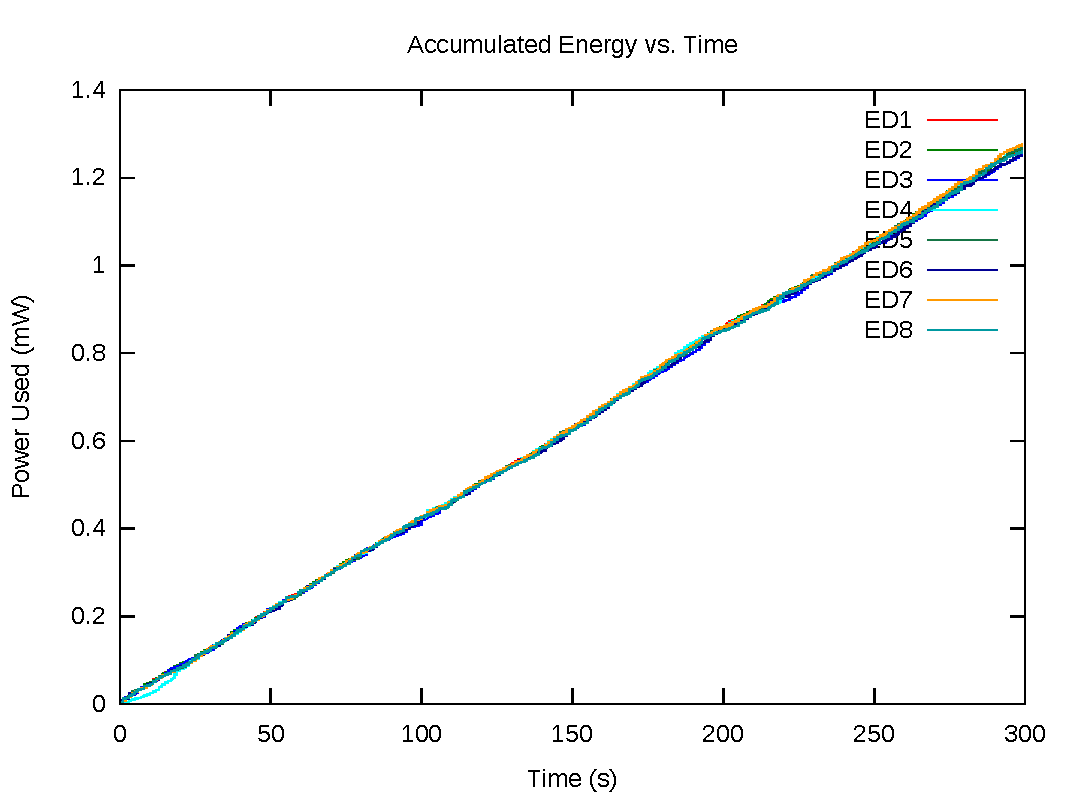
\includegraphics[width=0.5\textwidth]{figures/walk2-c100.pdf}
\end{center}
\caption{Walking (C=100)}
\label{fig:walk2-c100}
\end{figure}

\begin{figure}[htb]
\begin{center}
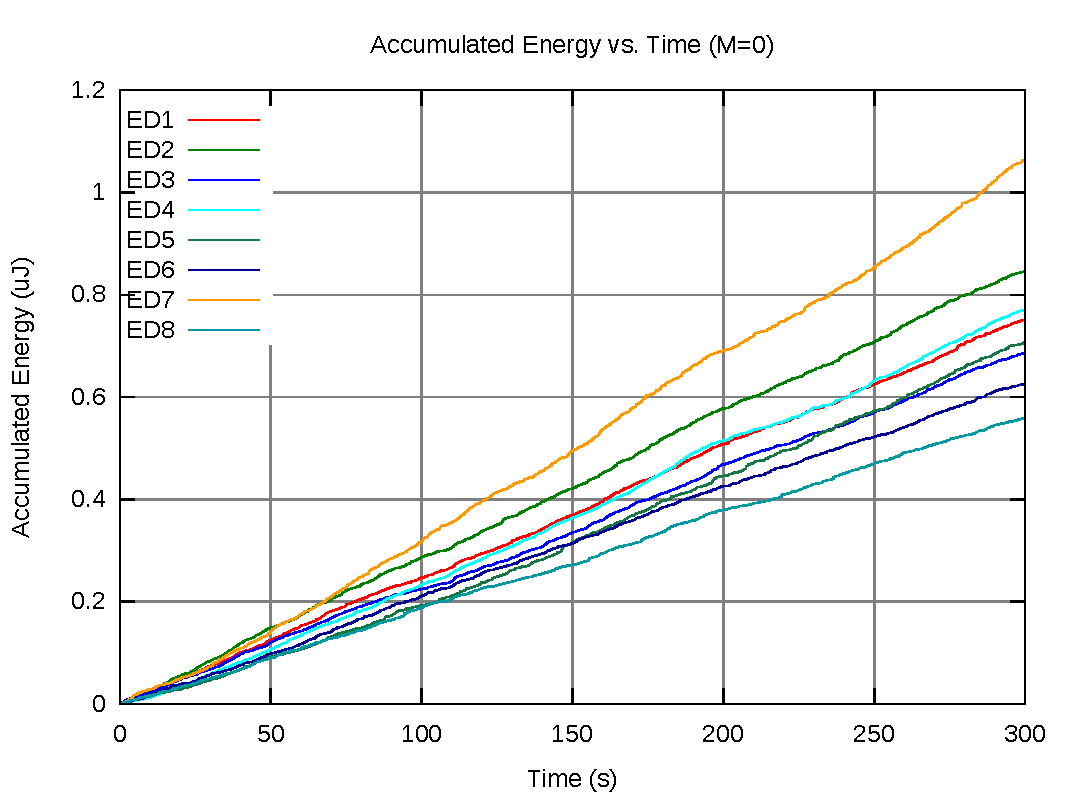
\includegraphics[width=0.5\textwidth]{figures/walk2-c0.pdf}
\end{center}
\caption{Walking (C=0)}
\label{fig:walk2-c0}
\end{figure}

$\ll$describe figure  3 and interpret results – network lifetime (like fig.8 in paper with Jeff)$\gg$ 

$\ll$describe figure  4 and interpret results – energy per bit (like fig.9 in paper with Jeff)$\gg$ 

$\ll$* maybe use CDFs?...$\gg$

\section{Conclusion}
$\ll$at the end: different from abstract -  The abstract in past tense + concentrate on meaning of results1

\bibliography{sources/thesis.bib}{}
\bibliographystyle{plain}
\end{document}